\section{Time-to-Empty Predictions}\label{sec:tte}

\subsection{Baseline scenarios}
For RP-63 (\cref{sec:params}), new, at 25\,$^\circ$C and from full charge, the nominal L2 TTE spans two orders
of magnitude, from 5.68\,h of gaming to 443\,h of Wi-Fi standby (\cref{tab:baseline}); for steady loads
$E_u/\bar P$ is at most 1.9\,\% too long (\cref{sec:analytic}). All these runs end at the cut-off with at most
1.1\,\% displayed, except the camera (brown-out in a 4\,W burst). The scheduled day S12 (9.5\,h screen-on from
07:00, including 1\,h of gaming; \cref{sec:usage}) dies on the second evening. Over 2048 parameter samples
(\cref{sec:uq}) the medians are 3\,\% (S12) to 38\,\% (S2b) shorter than nominal (\cref{sec:params}); only
gaming's is longer (16\,\%). Against published runtimes (\cref{fig:power_breakdown}b) and the Bonn data, room-temperature TTEs hold to
about $\pm15\,\%$ and cold ones are indicative (\cref{sec:wellpoor}).

\begin{table}[t]
\centering\small
\caption{TTE from full charge at 25\,$^\circ$C, new pack. $\bar P$: mean power (demand$\to$delivered if
throttled). TTE, event and $s_{\mathrm{off}}$ (displayed SOC at shutdown) are nominal; median and 90\,\% interval
over the parameter sample. Shares: two largest components of the demand (S7: before throttling; S12: of the
day's energy); proc.\ = processor (SoC). S13, S14: mean TTE; $^a$median and 5--95\,\% range over 2000 usage
paths; $^b$9.7 and 9.2\,\% brown-outs; CM was not sampled.}
\label{tab:baseline}
% Compact baseline TTE table (nominal values, parameter interval, component shares), generated from the
% scenario, uncertainty and power results (5-95 % parameter interval); numbers are not hand-edited.
% S13/S14 rows: full-model Monte Carlo over 2000 usage paths (mean, median, 5-95 % path quantiles).
\setlength{\tabcolsep}{3pt}%
\begin{tabular}{@{}llrrlrrl@{}}
\toprule
ID & Scenario & $\bar P$ (W) & TTE (h) & Median [90\,\%] (h) & Event & $s_{\mathrm{off}}$ (\%) & Top shares (\%) \\
\midrule
S1 & Standby, Wi-Fi & 0.040 & 443 & 373 [271, 584] & cut-off & 0.02 & floor 52, radio 48 \\
S2a & Standby, LTE & 0.047 & 378 & 348 [258, 519] & cut-off & 0.02 & radio 56, floor 44 \\
S2b & Standby, 5G, heavy push & 0.102 & 174 & 108 [81, 149] & cut-off & 0.04 & radio 79, floor 21 \\
S16 & Music, screen off, BT & 0.224 & 79.2 & 59.3 [41.0, 89.9] & cut-off & 0.09 & floor 49, audio 40 \\
S3 & Reading & 0.456 & 38.9 & 29.8 [22.7, 42.3] & cut-off & 0.18 & disp. 59, floor 24 \\
S5a & Video, Wi-Fi & 0.548 & 32.3 & 24.5 [19.3, 32.2] & cut-off & 0.21 & disp. 34, SoC 23 \\
S5b & Video, LTE & 0.694 & 25.5 & 20.4 [16.4, 25.9] & cut-off & 0.27 & radio 32, disp. 27 \\
S5c & Video, 5G NSA & 0.837 & 21.1 & 15.0 [12.3, 19.0] & cut-off & 0.32 & radio 43, disp. 23 \\
S4 & Social feed, Wi-Fi & 1.06 & 16.6 & 14.6 [11.7, 18.8] & cut-off & 0.40 & SoC 40, disp. 39 \\
S6 & Navigation & 1.49 & 11.8 & 10.3 [8.1, 13.4] & cut-off & 0.56 & disp. 34, SoC 29 \\
S8b & Video call, Wi-Fi & 1.62 & 10.8 & 8.6 [7.0, 11.2] & cut-off & 0.61 & SoC 35, radio 20 \\
CM & Camera & 1.69 & 10.4 & -- & brown-out & 0.68 & cam. 68, disp. 21 \\
S8a & Video call, LTE & 2.52 & 6.93 & 5.5 [4.1, 8.0] & cut-off & 0.93 & radio 48, SoC 22 \\
S7 & 3D gaming & 3.91$\to$3.06 & 5.68 & 6.6 [4.7, 9.0] & cut-off & 1.07 & SoC 81, disp. 11 \\
\midrule
S12 & Scheduled day & 0.528$\to$0.502 & 34.9 & 33.9 [25.2, 35.4] & cut-off & 0.93 & SoC 40, disp. 27 \\
S13 & Typical day (random) & 0.440 & 39.6 & 39.7 [27.8, 50.9]$^{a}$ & mixed$^{b}$ & 0.76 & -- \\
S14 & Heavy day (random) & 0.822 & 21.5 & 21.5 [13.5, 29.7]$^{a}$ & mixed$^{b}$ & 0.97 & -- \\
\bottomrule
\end{tabular}

\end{table}

\begin{figure}[t]
  \centering
  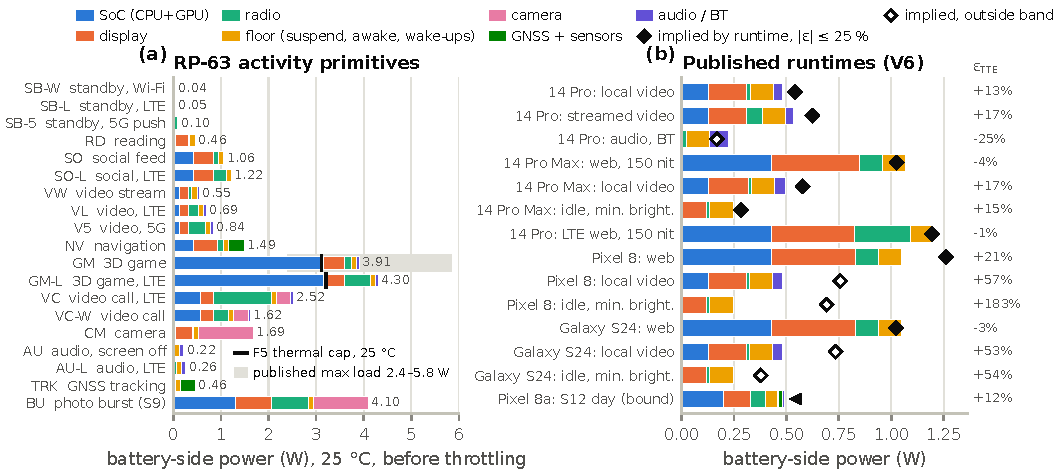
\includegraphics[width=0.95\textwidth]{figures/fig_power_breakdown.pdf}
  \caption{(a) Power by component before throttling; black tick: capped game power; grey band: published
  maximum loads \cite{NBC22,NBC23,NBC24}. (b) Model components for 14 published runtimes (V6); diamonds: power
  implied by the published runtime (filled: model within $\pm25\,\%$); triangle: lower bound (Pixel 8a);
  right: TTE error $\varepsilon_{\TTE}$.}
  \label{fig:power_breakdown}
\end{figure}

\subsection{Initial charge and SOC trajectories}\label{sec:initial}
At constant power SOC falls almost linearly, with the voltage knee only in the last few percent
(\cref{fig:trajectories}). TTE is therefore nearly proportional to the starting charge $s_0$ at 25\,$^\circ$C
(\cref{fig:tte_s0}a): for constant loads half a charge gives 0.471--0.477 of the full-charge TTE (typical random
day 0.49), matching the energy fraction at $s=0.5$ (0.477). On a coulombic display the last 20\,\% drains only
about 10\,\% faster than average, and on an energy gauge (which the Bonn data favour) evenly; there is no steep
``last 20\,\%''. Cold, aged packs are linear with an offset (\cref{fig:tte_s0}b): the chord through 50 and
100\,\% reaches zero at $s_0=12\,\%$ ($-10\,^\circ$C, SOH 0.8) and 25\,\% ($-20\,^\circ$C, where a cold-soaked phone
at $s_0\le25\,\%$ browns out at once). The cold hike ($-20\,^\circ$C, SOH 0.8) dies at its first or second photo
burst from $s_0\le45\,\%$. The scheduled day (0.34 from 50\,\%) depends on the time of day: its start time alone
moves the TTE between 27.9 and 42.8\,h.

\begin{figure}[t]
  \centering
  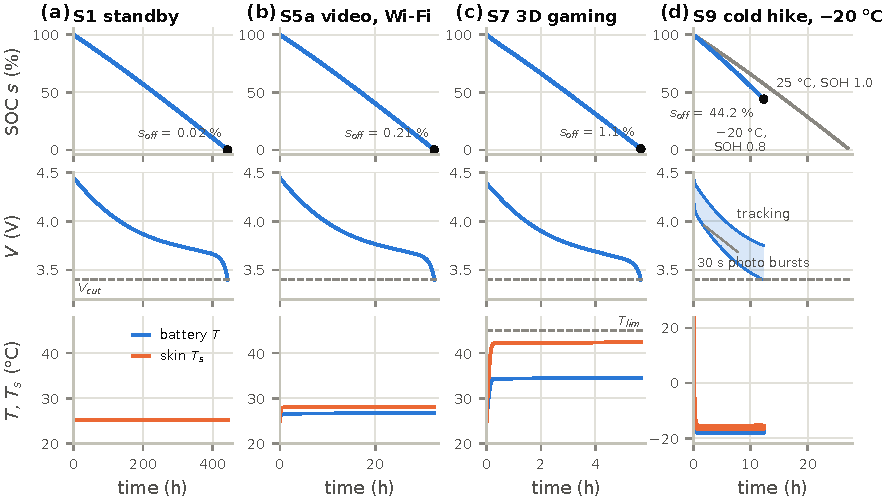
\includegraphics[width=0.66\textwidth]{figures/fig_trajectories.pdf}
  \caption{SOC, voltage and temperatures for constant loads and the cold hike. A game throttles within 10\,min.
  In (d) ($-20\,^\circ$C, SOH 0.8; grey: 25\,$^\circ$C, new) a photo burst ends the hike at 12.3\,h with 44\,\%
  still displayed. SOC paths of random days are shown in \cref{fig:ctmc}.}
  \label{fig:trajectories}
\end{figure}

\begin{figure}[t]
  \centering
  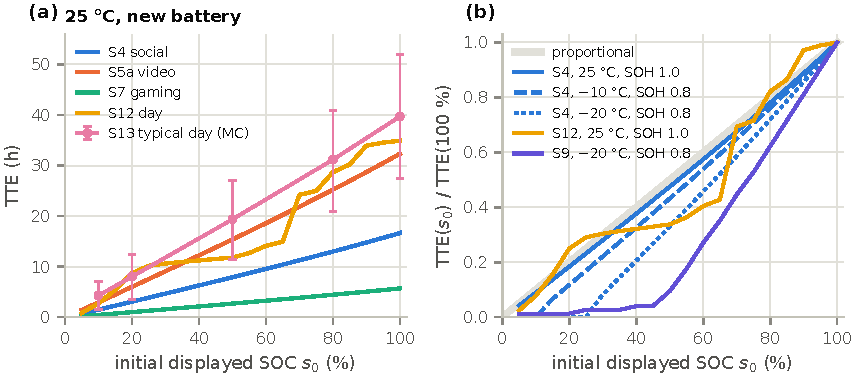
\includegraphics[width=0.7\textwidth]{figures/fig_tte_s0.pdf}
  \caption{(a) TTE against initial displayed SOC at 25\,$^\circ$C (S13: Monte Carlo (MC) mean, bars 5--95\,\% over usage paths).
  (b) TTE relative to full charge: cold, aged packs reach zero at a positive $s_0$.}
  \label{fig:tte_s0}
\end{figure}

\subsection{Drivers of rapid drain in each case}\label{sec:drivers}
For unthrottled loads the energy shares equal minus the TTE elasticities (F1), so \cref{tab:baseline} and
\cref{fig:power_breakdown}a name each driver. In standby the suspend floor and radio paging share the drain about
equally; heavy 5G push raises the radio share to 79\,\%. Reading and Wi-Fi video are display-bound, a 120\,Hz
social feed loads processor and display alike, cellular video and calls are radio-bound (32--48\,\%), and
navigation adds GNSS and sensors (21\,\%) to a bright screen. Gaming \emph{demand} is processor-bound (81\,\%
before throttling, 76\,\% of the delivered energy), but its TTE is set by the thermal cap: its elasticity to
$P_{\mathrm{SoC,max}}$ is only $-0.18$, to $R_{\mathrm{skin}}$ $+0.77$ (F5). Screen-off music pays as much for
keeping the processor awake (0.09\,W) as for audio and Bluetooth together. Over the scheduled day the shares are
processor 40.0, display 27.2, radio 14.5, awake 7.2, suspend 4.0, GNSS 3.4, audio 1.7, camera 1.3 and sensors
0.6\,\%, and its one hour of gaming uses about a quarter of the energy. Cold, aged packs die from resistance times
burst power.

\subsection{What reduces battery life most}\label{sec:most}
\textbf{(1) Sustained gaming}, capped by heat: throttling turns 3.91 into 3.06\,W at 0.85 performance and the game
lasts 5.68\,h; without throttling it would last 4.43\,h, and at 35\,$^\circ$C it lasts 10.3\,h but at only 0.52
performance (F5). Skipping one hour of it extends the typical day by 37\,\% (median 27\,\%, 90\,\%: 20--36\,\%),
the largest lever in every parameter sample. \textbf{(2) Cold, worse with age}: at $-20\,^\circ$C and SOH 0.8 the
social feed loses 39\,\% and the hike 54\,\% (12.3 instead of 27.0\,h at 25\,$^\circ$C, new), shutting down with
23 and 44\,\% still displayed. \textbf{(3) Cellular instead of Wi-Fi}: radio tails \cite{HU12,NA21} raise the
video radio share from 13 to 43\,\% (Wi-Fi to 5G); Wi-Fi gains 53\,\% (90\,\%: 34--102\,\%) for video and 56\,\%
for calls, and 5G push more than halves standby (174 vs.\ 378\,h on LTE). \textbf{(4) Poor coverage}: at
$-110$\,dBm the social feed on LTE loses 12\,\% (90\,\%: 5--35\,\%) and a video call 23\,\%; the Wi-Fi edge
($-90$\,dBm) costs 41\,\% \cite{DI13}, and a weak signal all day costs the typical day 5.7\,\%.
\textbf{(5) Bright, fast screens}: brightness $+0.2$ costs 7.5\,\% of the typical day; 60\,Hz and a dark theme
gain 4.7 and 4.6\,\% (\cref{sec:recs}).

\subsection{What changes battery life surprisingly little}\label{sec:least}
\textbf{Background sync:} halving wake-ups gains 0.1--0.4\,\% per day. \textbf{GNSS on a stationary phone:} a
Bonn iPhone 14 Pro lasts 48.5\,h with GPS against 55.0\,h idle \cite{SCH26,BONN26}, about 0.03\,W.
\textbf{Bluetooth:} 0.04\,W \cite{CH10}, 4\,\% of the social feed. \textbf{Sensors:} 0.3--0.6\,\% of a day's energy.
\textbf{Resistance at 25\,$^\circ$C:} losses of 0.41, 0.89 and 3.15\,\% at 0.5, 1.06 and 3.5\,W; its full prior
moves the social-feed TTE by at most 2\,\% (elasticity $-0.007$). \textbf{Cold on a fresh pack at moderate
load:} $-3.4\,\%$ (navigation) and $-2.7\,\%$ (social) at $-10\,^\circ$C, as the pack self-heats by 3--5\,K.
\textbf{Self-discharge:} 0.1\,\%/month \cite{ZIL19}. \textbf{Optimized charging:} +0.76 points of SOH in two years
(\cref{sec:aging}).

\begin{keybox}[Key finding]
At 25\,$^\circ$C TTE $\approx E_u/\bar P$: games, cellular radios and the screen decide drain; sync, GNSS,
sensors and resistance move a day by a few percent. Cold strands charge and age multiplies it (cold hike at
$-20\,^\circ$C: 17\,\% new, 44\,\% at SOH 0.8).
\end{keybox}
